\section{Base de datos}

\subsection{Estructura}

\subsubsection{Entidades}

En la \ref{fig:diagrama-e-r} se pueden localizar en color naranja las
entidades. En la siguiente lista se recogen los datos que almacenan cada una de
ellas.

\begin{description}
\item [Word] 
Palabras encontradas (en su norma normalizada o en su forma natural).

\item [Document]
Documentos procesados, con su t�tulo (entidad d�bil, forma clave con
Collection).

\item [DocType]
Tipos de documentos posibles (hasta el momento TRAIN y TEST). 

\item [Collection]
Colecciones completas procesadas y el nombre del fichero donde se encontraba.

\item [Property]
Todos los tags posibles, a nivel de palabra, clausal, frasal o de relaci�n
entre palabras.
	
\item [PropertyList]
Listas de elementos de tipo Property, para guardar los an�lisis a nivel frasal
y clausal.

\item [PropType]
Tipos de las propiedades (\begin{small}CLAUSE, WORD, PHRASE y
RELATIONSHIP\end{small}).
	
\item [Category]
Todas las categor�as encontradas.

\end{description}

\subsubsection{Relaciones}

La mayor�a de relaciones son bastante obvias mirando el diagrama
entidad-relaci�n por lo que en este apartado s�lo se van a comentar las que
tienen nombres que puedan inducir a confusi�n.

\begin{description}

\item [Syntactic]

\item [Semantic]

\end{description}

\begin{figure}[h]
\label{fig:diagrama-e-r}
\begin{center}
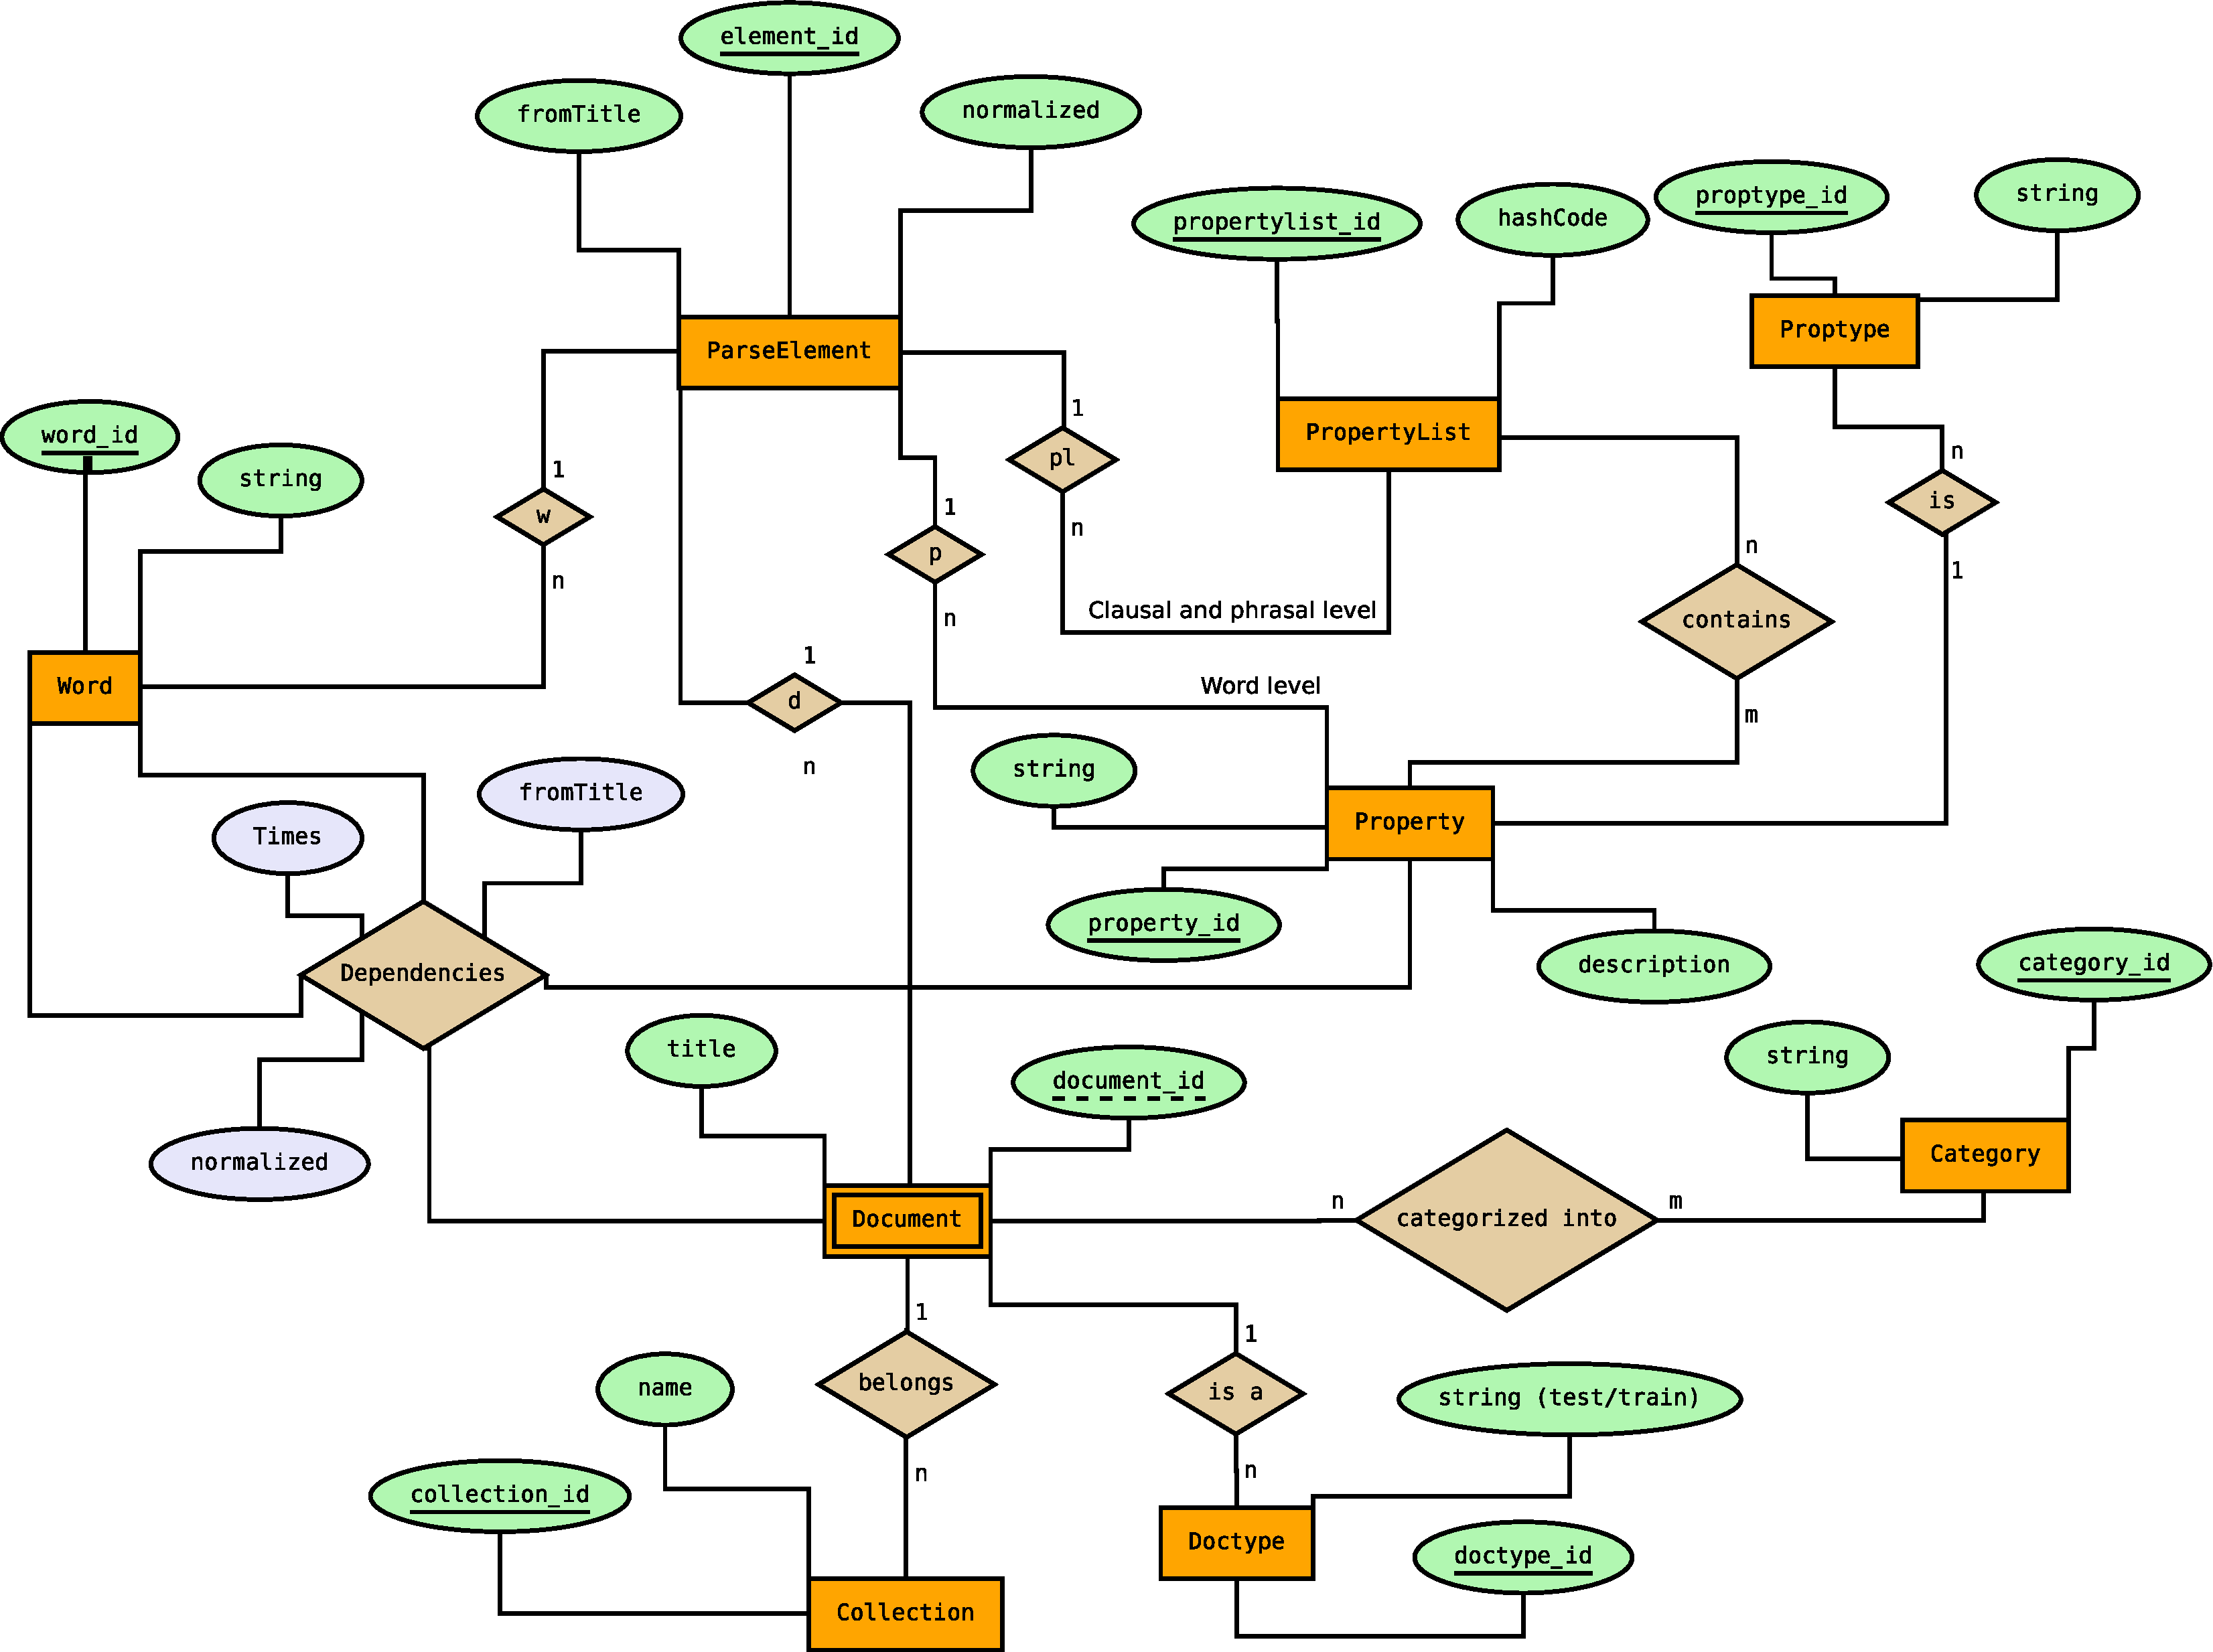
\includegraphics[angle=90,scale=0.425]{images/build/bdd-e-r.pdf}
\end{center}
\caption{Diagrama entidad-relaci�n de la base de datos}
\end{figure}

\subsection{Generaci�n de la base de datos}

MIEX es capaz de, mediante un fichero de texto con sentencas SQL, construir la
base de datos antes de empezar a procesar los ficheros de entrada (v�ase la
opci�n \textit{CreateDB} del fichero de configuraci�n). 

En el directorio \url{share/sql} est� situado el fichero de sentencias SQL
necesario para construir la base de datos que se comenta en esta secci�n, as�
como para insertar una serie de datos est�ticos necesarios.

\subsection{Normalizaci�n}

�Elena? FIXME

\subsection{Vistas}

Como se puede figurar despu�s de haber leido el primer cap�tulo, no es objetivo
del proyecto proporcionar un interfaz de consulta de la base de datos. De todos
modos, en el directorio \url{misc/query}, se pueden encontrar dos peque�os
scripts escritos en PHP\footnote{http://www.php.net} que contienen consultas de
ejemplo que pueden ser utilizadas como base bien para usuarios finales o bien
para futuras ampliaciones. Como breve explicaci�n, el programa
\textit{query.php} muestra una visi�n general de la base de datos, mientras que
el script \textit{showcat.php} permite hacer una b�squeda por categor�a.

Este par de herramientas han sido utilizadas fundamentalmente para hacer pruebas
de funcionamiento por lo que, adem�s de no considerarse funcionalidades
oficiales del proyecto, \textbf{se distribuyen sin ninguna garant�a
de funcionamiento}.

